% === C09 - Protección ===
% David Alejandro Gonzalez Marquez
% dmarquez@dc.uba.ar / fokerman@gmail.com
% https://github.com/fokerman/Orga2Course

\documentclass[aspectratio=169]{beamer}
% \documentclass[handout]{beamer}

% % % Packages
\usepackage[sfdefault]{AlegreyaSans}
\usepackage{inconsolata}
\usepackage{multicol}
\usepackage{multirow}
\usepackage[spanish]{babel}
\usepackage[utf8]{inputenc}
\usepackage{enumerate}
\usepackage{color}
\usepackage{xcolor}
\usepackage[absolute,overlay]{textpos}
  \setlength{\TPHorizModule}{1mm}
  \setlength{\TPVertModule}{1mm}
\usepackage{framed}
\usepackage{mfirstuc} % para poner en mayusculas la primer letra
\usepackage{xspace} % para crear espacios en comandos 
\usepackage{pbox}
\usepackage{tikz}
\usepackage{mathabx}

% % % Beamer config
\usetheme{Pittsburgh}
\usecolortheme[rgb={1,0.48,0.0}]{structure}
\setbeamercolor{block title}{fg=white,bg=verdeuca}
\xdefinecolor{verdeuca}{rgb}{0.0,0.48,0.54}
\xdefinecolor{naranjauca}{rgb}{1,0.48,0.0}
\setbeamercolor{palette quaternary}{fg=white,bg=verdeuca}
\setbeamertemplate{title page}[default][colsep=-4bp, rounded=true] % remove title shadow
\setbeamertemplate{frametitle}[default][colsep=-2bp, shadow=false] % remove frame title shadow
\setbeamertemplate{navigation symbols}{} % remove navigation symbols
\beamertemplatenavigationsymbolsempty

% % % Colors
\definecolor{AzulClaro}{rgb}{.31,.506,.741}
\definecolor{Gris}{gray}{0.8}
\definecolor{Celeste}{rgb}{.255,.41,.884}
\definecolor{Rojo}{rgb}{1, 0, 0}
\definecolor{a}{rgb}{0.0, 0.53, 0.74}
\definecolor{r}{rgb}{0.89, 0.0, 0.13}
\definecolor{v}{rgb}{0.0, 0.5, 0.0}
\definecolor{y}{rgb}{0.0, 0.5, 0.5}
\definecolor{rojo}{HTML}{F1521B}
\definecolor{verde}{HTML}{80CD29}
\definecolor{amarillo}{HTML}{FABC09}
\definecolor{azul}{HTML}{00ADF1}

% % % Rename
\newcommand{\tab}[0]{\hspace{15pt}}

% % % Blocks
\setbeamercolor{block body}{fg=black, bg=black!10}
\setbeamercolor{block title}{fg=black, bg=black!20}
\setbeamercolor{coloredboxstuffNaranja}{fg=naranjauca,bg=black!10} %% PARA LOS BOX
\setbeamercolor{coloredboxstuffVerde}{fg=verdeuca,bg=black!10} %% PARA LOS BOX

% % % Start

\title{\Huge Protección\\ \Large Niveles de privilegio y verificación de permisos}
\subtitle{Programación de Sistemas Operativos}
      
\author{David Alejandro González Márquez}
\institute{Departamento de Computación\\
Facultad de Ciencias Exactas y Naturales\\
Universidad de Buenos Aires}
\date{}

\begin{document}

\frame[plain]{\titlepage}

\begin{frame}{Introducción}
  \begin{itemize}
    \setlength\itemsep{0.8cm}
    \item[-] El objetivo de los mecanismos de protección en el procesador es:
    \vspace{0.3cm}
    \begin{itemize}
    \setlength\itemsep{0.3cm}
        \item[-] Restringir instrucciones. \pause
        \item[-] Limitar el acceso a la memoria. \pause
        \item[-] Limitar acciones sobre recursos. \pause
    \end{itemize}
    \item[-] En todos los sistemas operativos modernos se requiere minimamente\\ de dos niveles de protección: \textbf{Usuario} y \textbf{Supervisor}
  \end{itemize}
 \pause
  \vspace{0.5cm}
  Vamos a ver protección a nivel de \textbf{Segmentación}, \textbf{Paginación}, \textbf{Tareas} e \textbf{Interrupciones}.
\end{frame}

\begin{frame}[fragile]
    \frametitle{¿Donde configurar privilegios?}
    \begin{textblock}{100}(70,0.5) \only<3->{\includegraphics[scale=0.53]{img/usted_esta_aqui-layer2.pdf}} \end{textblock}
    \begin{textblock}{100}(70,0.5) \only<2->{\includegraphics[scale=0.53]{img/usted_esta_aqui-layer1.pdf}} \end{textblock}
    \begin{textblock}{100}(70,0.5) \only<1->{\includegraphics[scale=0.53]{img/usted_esta_aqui-layer3.pdf}} \end{textblock}
    \begin{textblock}{65}(3,17)
    \begin{enumerate}
    \setlength\itemsep{0.5cm}
    \small
     \item[-]<2-> \textcolor{naranjauca}{\texttt{DPL} - Descriptor Privilege Level:}\\ Parte de todas las entradas en tablas que describen memoria o estructuras del procesador.
     \item[-]<2-> \textcolor{naranjauca}{\texttt{RPL} - Requested Privilege Level:}\\ Parte de todos los selectores, permiten identificar descriptores. 
     \item[-]<2-> \textcolor{naranjauca}{\texttt{U/S} - User/Supervisor:}\\ Indican el nivel de privilegio en paginación.
    \end{enumerate}
    \end{textblock}
\end{frame}

\begin{frame}{Acceso a memoria}
    \begin{itemize}
    \setlength\itemsep{0.3cm}
    \item[-] Las unidades de segmentación y paginación transforman direcciones de memoria. \pause
    \item[-] Realizan las verificaciones de protección, determinando si el acceso puede o no realizarse. \pause
    \end{itemize}
    \begin{center}
    \Large Lógica $\xrightarrow[\text{Segmentación}]{}$ Lineal $\xrightarrow[\text{Paginación}]{}$ Física
    \end{center}

    \begin{itemize}
    \setlength\itemsep{0.1cm}
    \item[-] Lógica: \textcolor{verdeuca}{\texttt{selector:offset}} (16:32 bits)
    \item[-] Lineal: \textcolor{verdeuca}{\texttt{offset}} (32 bits)
    \item[-] Física: \textcolor{verdeuca}{\texttt{offset}} (32 bits)
    \end{itemize}
    \vspace{0.7cm}
    \footnotesize Nota: Suponiendo paginación no PAE, con paginas de 4k.
\end{frame}

\begin{frame}{Segmentación}
    \begin{textblock}{100}(75,0)
    \begin{center}
    Lógica $\xrightarrow[\textcolor{naranjauca}{\textbf{Segmentación}}]{}$ Lineal $\xrightarrow[\text{Paginación}]{}$ Física
    \end{center}
    \end{textblock}
    \begin{textblock}{100}(8,16)
    Estructuras necesarias para administrar segmentación.
    \end{textblock}
    \begin{textblock}{100}(10,25)
        \only<1->{\textcolor{verdeuca}{Selector de segmento}\\ \vspace{0.3cm}
        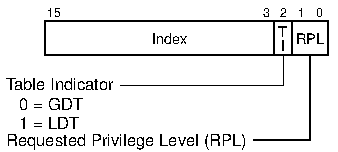
\includegraphics[scale=0.8]{img/segmentSelector.pdf}}
    \end{textblock}
    \begin{textblock}{100}(70,25)
        \only<1->{\textcolor{verdeuca}{Descriptor GDT}\\ \vspace{0.3cm}
        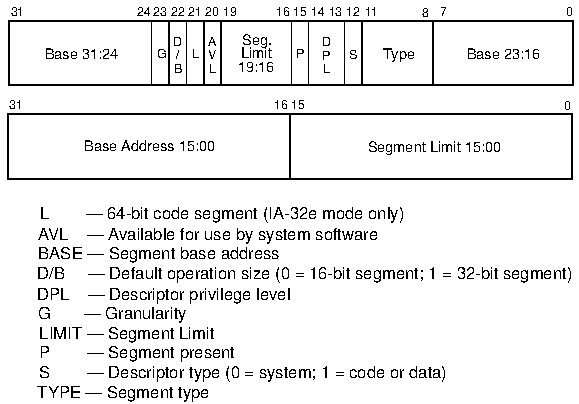
\includegraphics[scale=0.8]{img/segmentDescriptor.pdf}}
    \end{textblock}
\end{frame}

\begin{frame}{Segmentación}
    \begin{textblock}{100}(75,0)
    \begin{center}
    Lógica $\xrightarrow[\textcolor{naranjauca}{\textbf{Segmentación}}]{}$ Lineal $\xrightarrow[\text{Paginación}]{}$ Física
    \end{center}
    \end{textblock}
    Definiciones:
    \vspace{0.5cm}
    \begin{itemize}
    \setlength\itemsep{0.5cm}
        \item[-] \textcolor{naranjauca}{DPL (Descriptor Privilege Level)}:\\
        Nivel de privilegio del segmento para ser accedido (se ubica en su descriptor).
        \item[-] \textcolor{naranjauca}{RPL (Requested Privilege Level)}:\\
        Nivel de privilegio indicado en el selector de segmento como solicitud de acceso.
        \item[-] \textcolor{naranjauca}{CPL (Current Privilege Level)}:\\
        El \texttt{DPL} del segmento de código que se está ejecutando. Es nuestro nivel de privilegio.
        \item[-] \textcolor{naranjauca}{EPL (Effective Privilege Level)}:\\
        Máximo numérico entre el \texttt{CPL} y el \texttt{RPL}, es decir, 
        \texttt{EPL=max(CPL,RPL)}
    \end{itemize}
\end{frame}

\begin{frame}{Segmentación}
    \begin{textblock}{100}(75,0)
    \begin{center}
    Lógica $\xrightarrow[\textcolor{naranjauca}{\textbf{Segmentación}}]{}$ Lineal $\xrightarrow[\text{Paginación}]{}$ Física
    \end{center}
    \end{textblock}
    Verificación direcciones $\rightarrow$ \textcolor{verdeuca}{\texttt{selector:offset}}
    \vspace{0.1cm}
    \begin{enumerate}
    \setlength\itemsep{0.2cm}
    \item<2->[1.] Verificar que el segmento este presente (\texttt{P=1}).
    \item<3->[2.] Verificar límite del segmento.
        \begin{itemize}
        \item[-] Si \texttt{G=0}: \texttt{offset < (segment.limit+1)}
        \item[-] Si \texttt{G=1}: \texttt{offset < (segment.limit+1) * 0x1000}
        \end{itemize}
    \item<4->[3.] Verificar el nivel para acceder al segmento. {\scriptsize (Las comparaciones $=$, $\geq$, $\leq$ son por valor numérico)}
        \begin{itemize}
        \item<4->[-] Si el segmento es de datos \texttt{$\rightarrow$} \texttt{EPL} $\leq$ \texttt{DPL}
        \item<5->[-] Si es un segmento de código:
        \begin{itemize}
        \item[-] Non-conforming \texttt{$\rightarrow$} \texttt{CPL} $=$ \texttt{DPL}
        \item[-] Conforming \texttt{$\rightarrow$} \texttt{CPL} $\geq$ \texttt{DPL}
        \end{itemize}
        \end{itemize}
    \item<6->[4.] Verificar acción a realizar
        \begin{itemize}
        \item<7->[-] Leer: Cualquier segmento de datos, restringido en segmentos de código.
        \item<8->[-] Escribir: Restringido en segmentos de datos, prohibido en segmentos de código.
        \item<9->[-] Ejecutar: Permitido solo en segmentos de código.
        \end{itemize}
    \end{enumerate}
    \vspace{0.1cm}
    \uncover<10->{\small Si alguna de las verificaciones falla: \texttt{$\rightarrow$ General Protection Fault (\#GP)}}
\end{frame}

\begin{frame}{Segmentación}
    \begin{textblock}{100}(75,0)
    \begin{center}
    Lógica $\xrightarrow[\textcolor{naranjauca}{\textbf{Segmentación}}]{}$ Lineal $\xrightarrow[\text{Paginación}]{}$ Física
    \end{center}
    \end{textblock}
    \begin{textblock}{100}(20,12)
        Tipos de segmentos de código o datos\\
        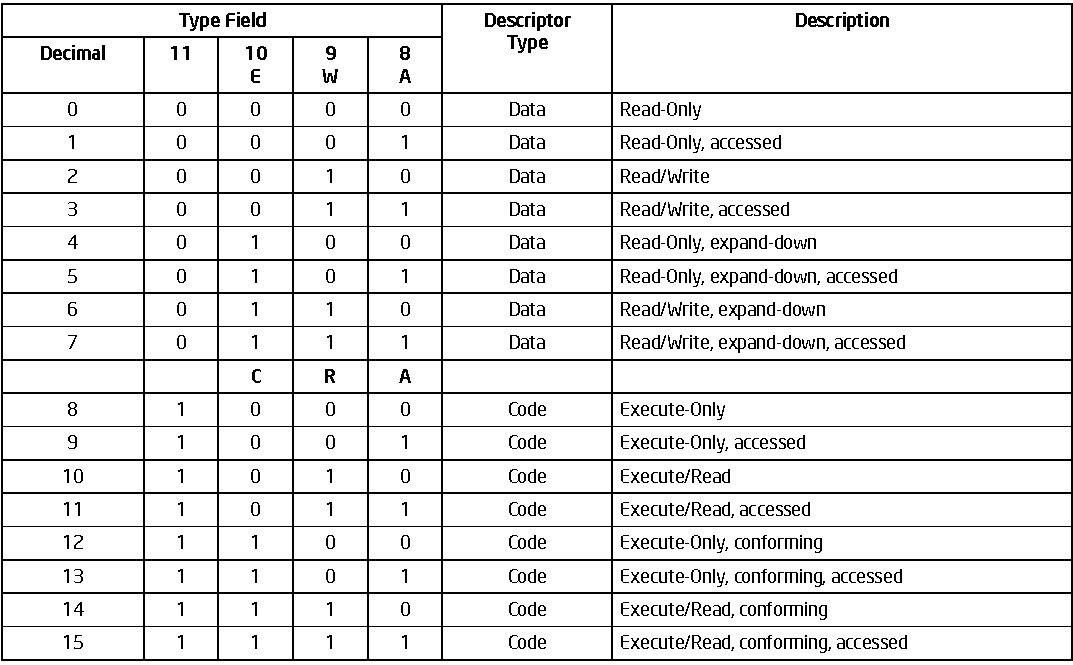
\includegraphics[scale=0.64]{img/typeTable.pdf}
    \end{textblock}
\end{frame}

\begin{frame}{Paginación}
    \begin{textblock}{100}(75,0)
    \begin{center}
    Lógica $\xrightarrow[\text{Segmentación}]{}$ Lineal $\xrightarrow[\textcolor{naranjauca}{\textbf{Paginación}}]{}$ Física
    \end{center}
    \end{textblock}
    \begin{textblock}{140}(12,17)
    Las direcciones en paginación son resueltas por medio de directorios y tablas de paginas.\\
    El nivel de acceso está dado por atributos en las entradas de estas tablas (\texttt{PDE} y \texttt{PTE}).
    \end{textblock}
    \begin{textblock}{100}(35,30) 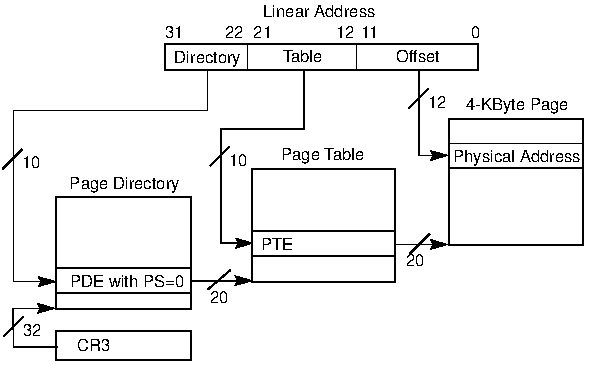
\includegraphics[scale=0.85]{img/paging.pdf} \end{textblock}
\end{frame}

\begin{frame}{Paginación}
    \begin{textblock}{100}(75,0)
    \begin{center}
    Lógica $\xrightarrow[\text{Segmentación}]{}$ Lineal $\xrightarrow[\textcolor{naranjauca}{\textbf{Paginación}}]{}$ Física
    \end{center}
    \end{textblock}
    Verificación direcciones $\rightarrow$ \textcolor{verdeuca}{\texttt{lineal}} $\rightarrow$ \textcolor{verdeuca}{\texttt{PDindex:PTindex:offset}}
    \vspace{0.1cm}
    \begin{enumerate}
    \setlength\itemsep{0.2cm}
    \item<2->[1.] Verificar que la pagina este presente (\texttt{PDE.P=1} y \texttt{PTE.P=1}).
    \item<3->[2.] Verificar el nivel para acceder a la página.
        \begin{itemize}
        \item<4->[-] Si \textcolor{verdeuca}{\texttt{PDE.US=0} \texttt{or} \texttt{PTE.US=0} } la página tiene permisos de supervisor (\texttt{CPL=0 o 1 o 2}).
        \item<5->[-] Si \textcolor{verdeuca}{\texttt{PDE.US=1} \texttt{and} \texttt{PTE.US=1}} la página tiene permisos de usuario (\texttt{CPL=3}).
        \end{itemize}
    \item<6->[3.] Verificar acción a realizar
        \begin{itemize}
        \item<7->[-] Leer: Cualquier pagina puede ser leída.
        \item<8->[-] Ejecutar: Cualquier pagina puede ser ejecutada.
        \item<9->[-] Escribir: 
        \begin{itemize}
        \item<9->[-] Si \textcolor{verdeuca}{\texttt{PDE.RW=0} \texttt{or} \texttt{PTE.RW=0} } la página no puede ser escrita.
        \item<10->[-] Si \textcolor{verdeuca}{\texttt{PDE.RW=1} \texttt{and} \texttt{PTE.RW=1}} la página puede ser escrita.
        \end{itemize}
        \end{itemize}
    \end{enumerate}
    \vspace{0.3cm}
    \uncover<11->{\small Si alguna de las verificaciones falla: \texttt{$\rightarrow$ Page Fault (\#PF)}}
\end{frame}

\begin{frame}{Paginación}
    \begin{textblock}{100}(75,0)
    \begin{center}
    Lógica $\xrightarrow[\text{Segmentación}]{}$ Lineal $\xrightarrow[\textcolor{naranjauca}{\textbf{Paginación}}]{}$ Física
    \end{center}
    \end{textblock}
    \begin{textblock}{100}(20,12)
        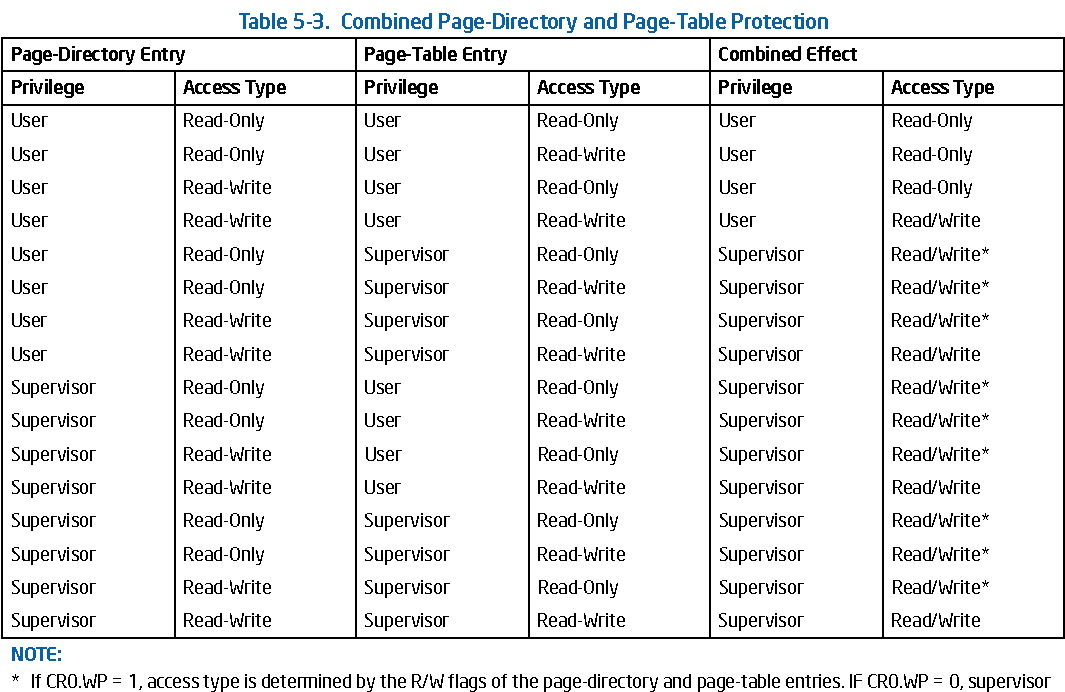
\includegraphics[scale=0.64]{img/combinacionPDPT.pdf}
    \end{textblock}
\end{frame}

\begin{frame}{Intercambio de tareas}
    \begin{textblock}{65}(5,17)
        \begin{itemize}
        \setlength\itemsep{0.3cm}
        \small
        \item[-] El \texttt{DPL} de los descriptores de \texttt{TSS} indica el nivel de privilegio necesario para ejecutar la tarea.
        \item<2->[-] Verificar si es posible saltar a una tarea:
        \vspace{0.2cm}
        \begin{enumerate}
        \small
        \setlength\itemsep{0.2cm}
        \item<3->[1.] Verificar TSS presente: \texttt{P=1}.
        \item<4->[2.] Verificar privilegios: \texttt{CPL $\leq$ DPL}
        \item<5->[3.] Verificar bit \texttt{Busy} en cero.
        \end{enumerate}
        \end{itemize}
        \vspace{0.5cm}
        \uncover<6->{\small Si alguna de las verificaciones falla:\\ \texttt{$\rightarrow$ General Protection Fault (\#GP)}}
    \end{textblock}
    \begin{textblock}{100}(75,12)
        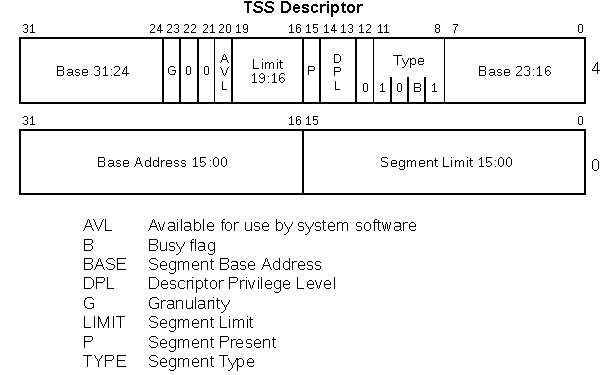
\includegraphics[scale=0.8]{img/TSSdescriptor.pdf}
    \end{textblock}
\end{frame}

\begin{frame}{Interrupciones}
    \begin{textblock}{100}(85,0) 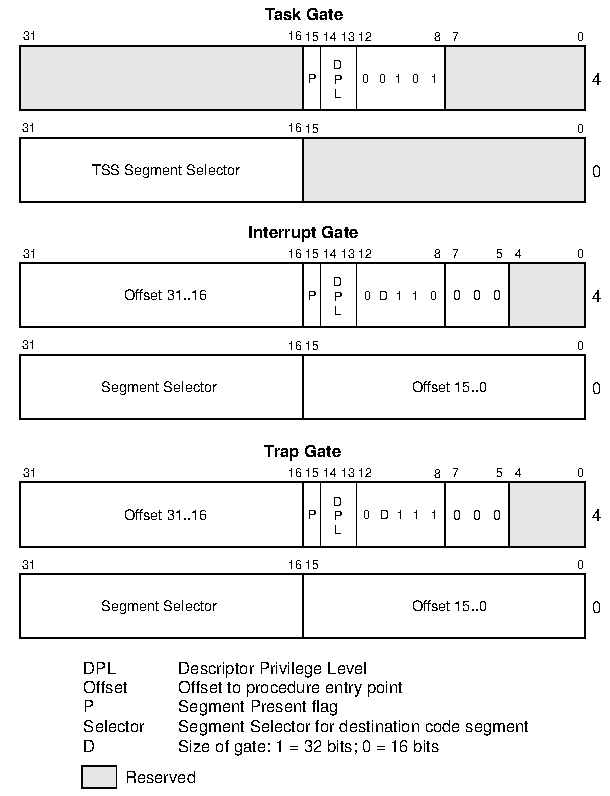
\includegraphics[scale=0.7]{img/interruptsGates.pdf} \end{textblock}
    \begin{textblock}{70}(5,15)
    \textcolor{verdeuca}{Descriptores de IDT}\\
    \begin{itemize}
     \item[-] Cada entrada de interrupciones tiene su propio \texttt{DPL}.
     \item[-] Indica el nivel de privilegio necesario para poder acceder a la interrupción.
    \end{itemize}
    \end{textblock}
\end{frame}

\begin{frame}{Interrupciones}
    Verificación de privilegios para generar una interrupción.
    \vspace{0.5cm}
    \begin{enumerate}
    \setlength\itemsep{0.4cm}
    \item<2->[1.] Verificar que la interrupción esté presente $\rightarrow$ \texttt{P=1}.
    \item<3->[2.] Verificar el nivel para acceder a la interrupción
    \begin{itemize}
     \item<4->[-] Si la interrupción es generada por código: $\rightarrow$ \texttt{DPL} $\geq$ \texttt{CPL}
     \item<5->[-] Si la interrupción es generada externamente: No se verifica.
     \item<6->[-] Si la interrupción es una excepción del procesador: No se verifica.
    \end{itemize}
    \end{enumerate}
    \vspace{0.5cm}
    \uncover<7->{\small Si alguna de las verificaciones falla: \texttt{$\rightarrow$ General Protection Fault (\#GP)}}
\end{frame}

\begin{frame}[fragile]
    \frametitle{Bibliografía: Fuentes y material adicional}
    \begin{itemize}
    \item Convenciones de llamados a función en x86: \\
    \url{https://en.wikipedia.org/wiki/X86_calling_conventions}
    \item Notas sobre System V ABI: \\
    \url{https://wiki.osdev.org/System_V_ABI}
    \item Documentación de NASM: \\
    \url{https://nasm.us/doc/}
    \item Artículo sobre el flag \texttt{-pie}: \\
    \url{https://eklitzke.org/position-independent-executables}
    \item Documentación de System V ABI: \\
    \url{https://uclibc.org/docs/psABI-x86_64.pdf}
    \item Manuales de Intel: \\
    \url{https://software.intel.com/en-us/articles/intel-sdm}
    \end{itemize}
\end{frame}

\begin{frame}[plain]
    \begin{center}
    \vspace{2cm}
    \huge ¡Gracias!\\
    \vspace{2cm}
    \normalsize Recuerden leer los comentarios al final de \\ este video por aclaraciones o fe de erratas.
    \end{center}
\end{frame}

\end{document}
